The dendrogram view shows the result of a hierarchical clustering.
A hierarchical clustering works on a (sub)set of molecules and a couple of properties.
In the beginning, the clustering algorithm puts each molecule into one cluster. Then it searches for two molecules (clusters) with the smallest distance between each other based on the chosen properties.
When found, they are merged into a new cluster. 
This will be repeated until only one cluster remains.
The result is a tree which represents the merge history like shown in \figref{fig:dendrogram_tree}.

The dendrogram view shows this result, allows the user to navigate in the hierarchical tree structure and to highlight different clusters based on their relation.

\begin{figure}[!htb]
\centering
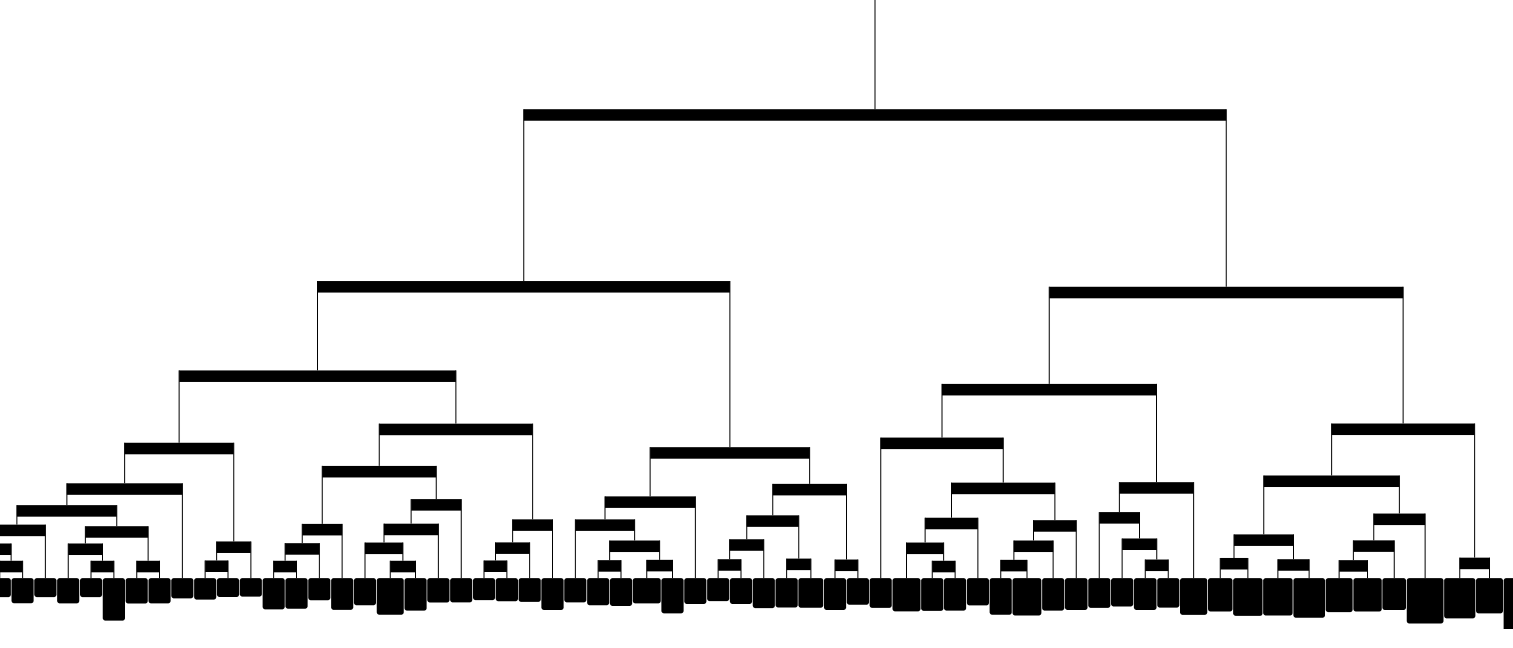
\includegraphics[width=1\textwidth]{images/dendrogram/dendrogram}
\caption{The tree frame}
\label{fig:dendrogram_tree}
\end{figure}

\subsection{The View in Detail}

The dendrogram view is separated in four parts, shown in \figref{fig:dendrogram_regions}. Each part is marked by a surrounding color as explained below:
\begin{itemize}
\item the tree frame in which the result is shown  (marked yellow)
\item the \sbar (marked red) 
\item the \tbar (marked blue)
\item a special representation of the table view (marked green)
\end{itemize}

 \begin{figure}[!htb]
\centering
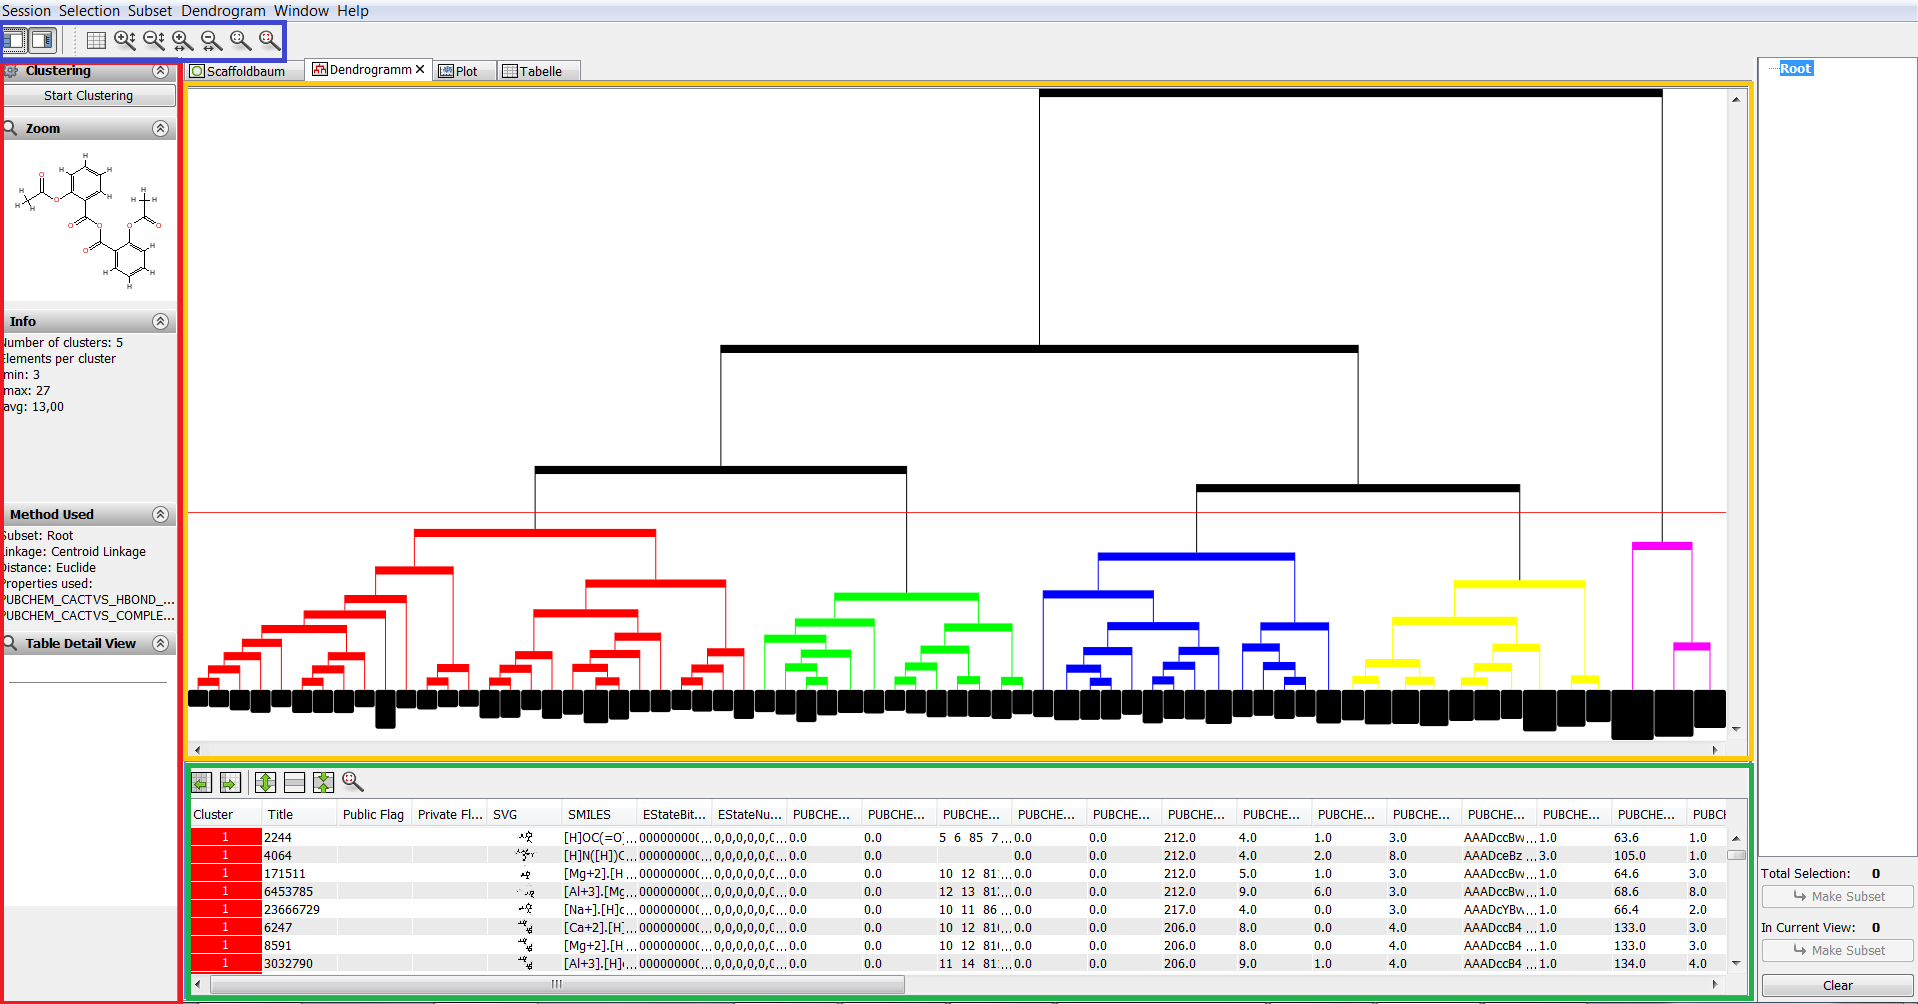
\includegraphics[width=1\textwidth]{images/dendrogram/overview_with_marks}
\caption{The whole view}
\label{fig:dendrogram_regions}
\end{figure} 

\subsection{Side Bar}

% \begin{figure}[!htb]
%\centering
%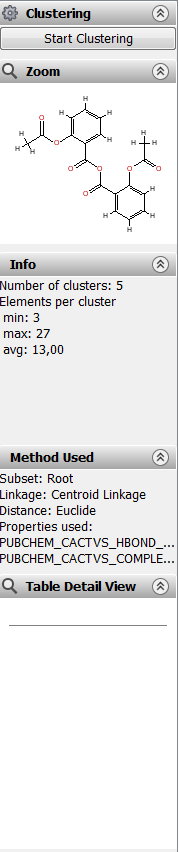
\includegraphics[width=0.1\textwidth]{images/dendrogram/sidebar}
%\caption{The Sidebar}
%\label{fig:dendrogram_sidebar}
%\end{figure} 
\figref{fig:dendrogram_regions} shows the dendrogram \sbar (marked red). 
\begin{itemize}
\item The \gui{Start Clustering} button opens the configuration dialog for the clustering
\item The \gui{Zoom} element shows the molecule under the mouse in detail
\item The \gui{Info} element shows statistical data about the currently chosen clustering
\item The \gui{Method Used} element shows which configuration was used to generate the actual dendrogram
\item The \gui{Table Detail} element is equal to its correspondent in the real table view
\end{itemize}



\subsection{Tree Frame} 

%\begin{figure}[!htb]
%\centering
%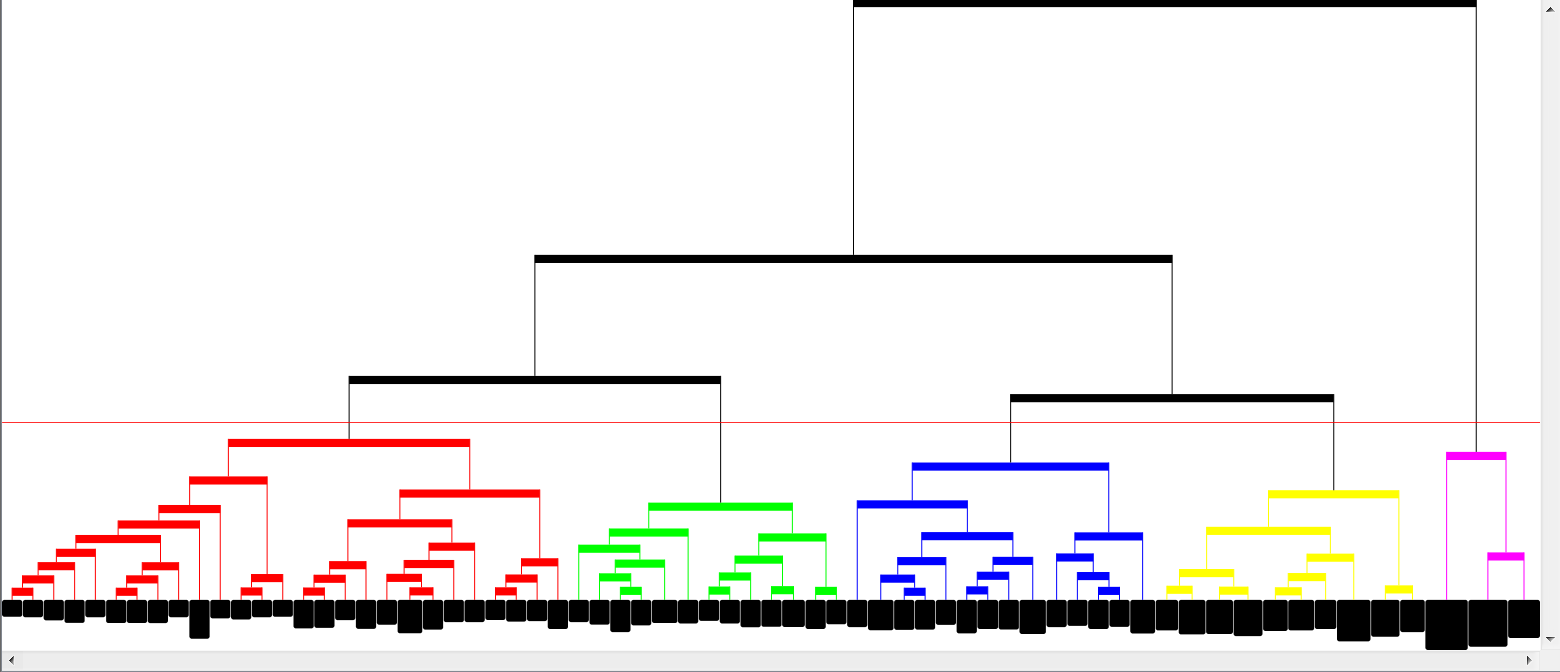
\includegraphics[width=0.8\textwidth]{images/dendrogram/main}
%\caption{The tree frame}
%\label{fig:dendrogram_tree}
%\end{figure}



In this part of the view you can see an actual dendrogram like shown in \figref{fig:dendrogram_tree}.
The molecules on the bottom are represented by black boxes because the zoom level is too small to show the real images.
The cluster selection bar shown in red in the middle is draggable and divides the subtrees below it into different clusters.
Each cluster separated this way is painted in a different own color.
The Info panel in the \sbar informs about the number of clusters created this way and their size.
With the mouse wheel or the keys “+” and “-“ the view can be zoomed in and out.
At a closer zoom level the black boxes at the bottom are replaced by the real molecule images like shown in \figref{fig:dendrogram_regions} (marked yellow). 

\begin{figure}[!htb]
\centering
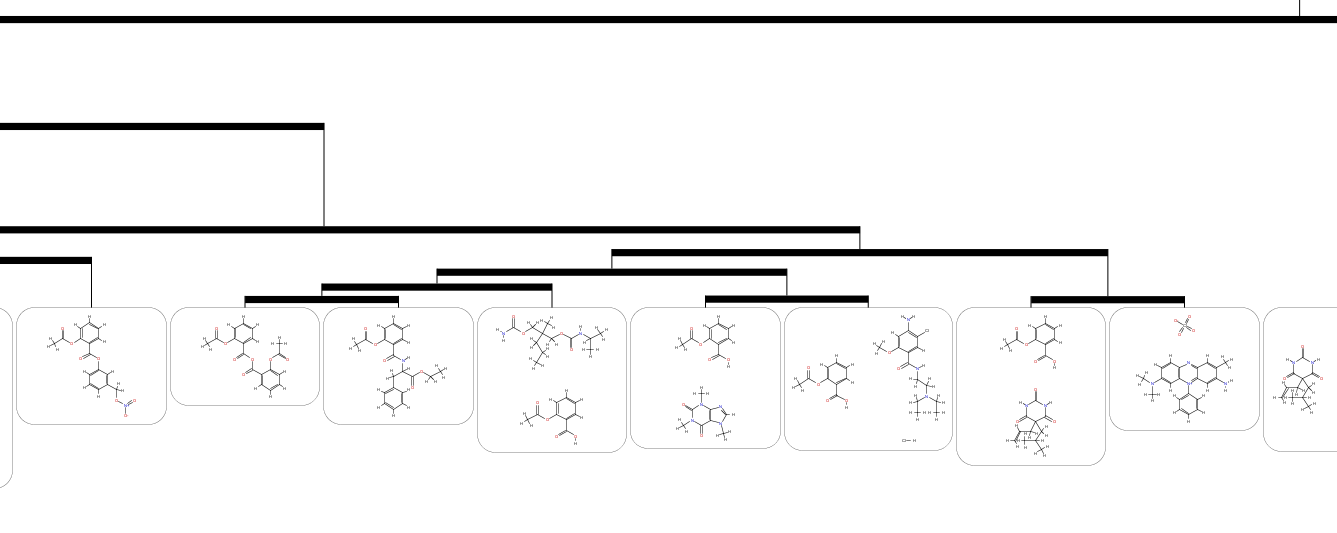
\includegraphics[width=0.8\textwidth]{images/dendrogram/zoomin}
\caption{Zoomed in}
\label{fig:dendrogram_zoom}
\end{figure} 

The zoom is separated into vertical and horizontal zoom.
This is necessary, because the tree usually has a very small height and a huge width.
So when zooming with the mouse wheel, the view scales the images and than adapts the tree above to fit in the window.
Zooming while holding the \texttt{Ctrl} key will scale only the tree, not the image. 
In addition to click on an image to add/remove it from the selection,
clicking on an inner node of the tree will result in selecting all leaves below it,
if at least one leaf is unselected and deselect them otherwise.


\subsection{Tool Bar}
 \begin{figure}[!htb]
\centering
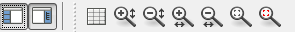
\includegraphics[width=0.5\textwidth]{images/dendrogram/toolbar}
\caption{The \tbar}
\label{fig:dendrogram_tool}
\end{figure} 
The two buttons on the left shown in \figref{fig:dendrogram_tool} are the standard items to show/hide the side- and subset bar.
The third button  from the left shows/hides a special table below the dendrogram.
The next four buttons change the vertical and horizontal zoom of the dendrogram.
The second button from the right fits the dendrogram into the available space.
The button at the right zooms the view so that the whole selection is visible.


\subsection{Table}
% \begin{figure}[!htb]
%\centering
%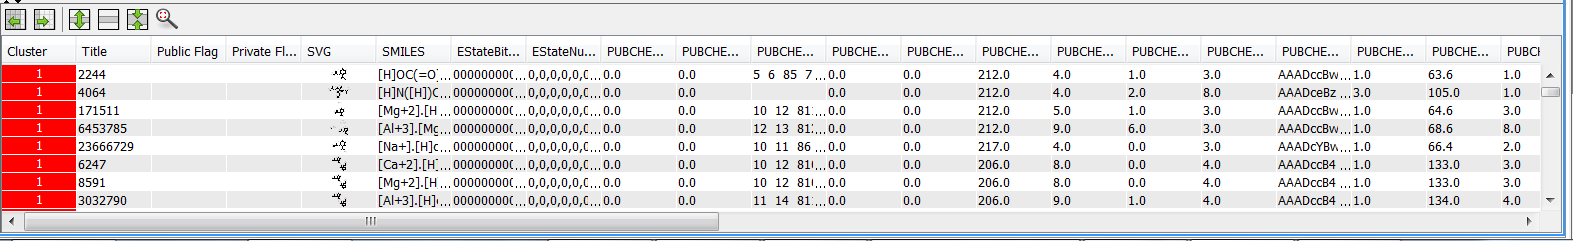
\includegraphics[width=1\textwidth]{images/dendrogram/table}
%\caption{The table below the dendrogram}
%\label{fig:dendrogram_table}
%\end{figure} 
The shown table below the dendrogram is the standard table view with one additional function, see \secref{sec:scaffoldhunter:table}.
The first column shows in which subclusters the selection bar in the dendrogram has divided the molecules.
An example is shown in \figref{fig:dendrogram_regions} (marked green).


\subsection{Clustering Configuration Panel}
\begin{figure}[!htb]
\centering
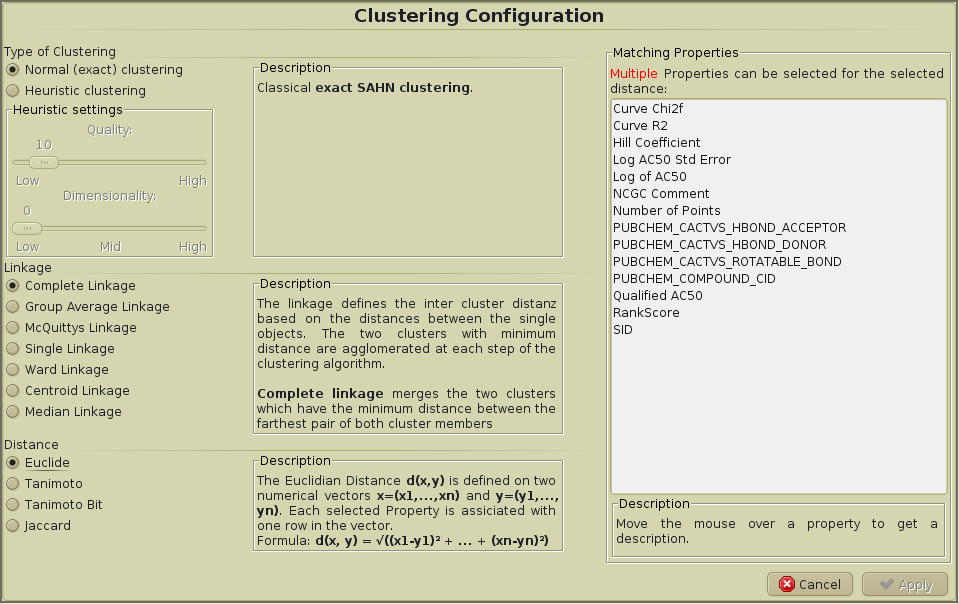
\includegraphics[width=0.9\textwidth]{images/dendrogram/clusteringConfig}
\caption{The clustering config dialog}
\label{fig:dendrogram_config}
\end{figure}
After clicking the start clustering button in the \sbar, a configuration panel as in \figref{fig:dendrogram_config} will show up.
Here, the user can choose from two clustering algorithms and select their parameters:

\subsubsection{Clustering Algorithms}
\paragraph{Normal (exact) clustering:} 
Classical exact SAHN clustering.

\warningbox{Warning}{The exact clustering can work on $2^{16}$ (65.536) molecules at a max, because of technical restrictions in Java and memory limitation.
Some of the parameters (\textit{Euclide} in combination with \textit{Ward, Median} or \textit{Centroid}) may work on more molecules, but this is experimental and should only be used with caution.
Please note that these restrictions do not apply to the heuristic algorithm.}

\paragraph{Heuristic clustering:} 
   The heuristic SAHN clustering algorithm should be 
   used if the runtime or the memory consumption by the exact clustering is to 
   high. Empiric tests showed that this algorithm can be considered useful for 
   subsets with a size larger that 10000 molecules. Two parameters are selectable:
   quality and dimensionality. Both have a direct influence on quality and speed.
   The dimensionality should be set according to the dimensionality of the data.
   Low for a dimensionality between 1 and 7, Mid 7-13 and High $>$ 13. If unsure
   start with a low dimensionality and use a higher value if the quality is 
   insufficient regardless of which quality is used.   


\subsubsection{Linkage \& Distance} \label{sec:scaffoldhunter:clustering:parameters}
The linkage method defines the way in which the distance between clusters is calculated and controls which pair should be merged.

\begin{itemize}

\item \textbf{Complete Linkage:} Merges the two clusters which have the minimum distance between the farthest pair of both cluster members.
\item \textbf{Group Average Linkage:} Merges the two clusters with the minimum distance of the unweighted cluster average (UPGMA).
\item \textbf{McQuittys Linkage}: Merges the two clusters with the minimum distance of the weighted cluster average (WPGMA).
\item \textbf{Single Linkage:} Merges the two clusters with the minimum distance between the nearest pair of both cluster members.
\item \textbf{Ward Linkage:} Merges the two clusters that lead to minimal variance increase.
\item \textbf{Centroid Linkage}: Merges the two clusters with the minimum distance of the unweighted centers (UPGMC).
\item \textbf{Median Linkage:} Merges the two clusters with the minimum distance of the weighted cluster centers (WPGMC).

\end{itemize}
The accepted types of properties depend on the distance computation.
\begin{itemize}

\item \textbf{Euclide:} Any number of numerical properties.
\item \textbf{Tanimoto:} Exactly one property which has to be a binary fingerprint.
\item \textbf{Tanimoto Bit:} Same as Tanimoto but works on bit strings not on character strings.
\item \textbf{Jaccard:} Works on one fingerprint property with feature counts on each position.
\end{itemize}

